
%----------------------------------------------------------------------------------------
% Lecture: Old Keynesian Model (AD in (x,pi) + backward-looking Phillips + policy rule)
% TikZ figures included (no external images required)
% Template style: SimpleDarkBlue + itemize/enumerate (no heavy boxes)
%----------------------------------------------------------------------------------------

\documentclass[aspectratio=169,xcolor=dvipsnames]{beamer}
\usetheme{SimpleDarkBlue}

\usepackage{hyperref}
\usepackage{graphicx}
\usepackage{booktabs}
\usepackage{appendixnumberbeamer}
\usepackage{amsmath}
\usepackage{iftex}
\usepackage{tikz}
\usetikzlibrary{arrows.meta,calc}

% --- Font handling (compile anywhere) ---
\ifPDFTeX
  \usepackage[T1]{fontenc}
  \usepackage{lmodern}
  \usepackage{microtype}
\else
  \usepackage{fontspec}
  \usepackage{luatexja}
  \setmainfont{Alegreya Sans Light}[
    ItalicFont={* Italic},
    BoldFont={Alegreya Sans Medium},
    BoldItalicFont={Alegreya Sans Medium Italic}]
  \setsansfont{Alegreya Sans Light}[
    ItalicFont={* Italic},
    BoldFont={Alegreya Sans Medium},
    BoldItalicFont={Alegreya Sans Medium Italic}]
\fi

% --------------------------- %
% Section title page with toc %
% --------------------------- %
\setbeamertemplate{subsection page}{%
    \usebeamertemplate*{section page}
}
\setbeamertemplate{section in toc}[square]
\setbeamertemplate{subsection in toc}[square]
\AtBeginSection[]{
% \sepframe
\begin{frame}[noframenumbering]{Outline}
    % \tableofcontents[currentsection]
    \tableofcontents[currentsection, currentsubsection]
\end{frame}
}
\AtBeginSubsection[]{
  \begin{frame}[noframenumbering]{Outline}
    \tableofcontents[currentsection, currentsubsection]
  \end{frame}
}

% % ------------------------------------ %
% % Section title page with Huge bf text %
% % ------------------------------------ %
% \AtBeginSection[]{
%   \begin{frame}[noframenumbering, plain]
%     \Huge{\centerline{\textbf{\insertsection}}}
%   \end{frame}
% }

%%% automatically add spaces into enumerate and itemize environment
\let\tempone\itemize
\let\temptwo\enditemize
\renewenvironment{itemize}{\tempone\addtolength{\itemsep}{\fill}}{\temptwo}
\let\tempa\enumerate
\let\tempb\endenumerate
\renewenvironment{enumerate}{\tempa\addtolength{\itemsep}{\fill}}{\tempb}

%%=============================================================
%%  FOOTLINE TEMPLATE
%%=============================================================
\defbeamertemplate*{footline}{shadow theme}{%
    \leavevmode\hbox{%
        \hypersetup{linkcolor=white,urlcolor=white,citecolor=white}
        \begin{beamercolorbox}[wd=1.02\paperwidth, ht=2.5ex, dp=1.125ex,
          leftskip=.3cm plus1fil, rightskip=0.3cm]{author in head/foot}%
            \insertsectionnavigationhorizontal{.80\textwidth}{}{} \hspace{.3cm}
            \hfill \#\ \insertframenumber \ / \ \inserttotalframenumber%
        \end{beamercolorbox}%
    }%
}
\setbeamertemplate{footline}[shadow theme]

%----------------------------------------------------------------------------------------
%    TITLE PAGE
%----------------------------------------------------------------------------------------
\title[Old Keynesian]{Macroeconomics II (Spring 2026)\\\vspace{4pt}Old Keynesian Model: AD + Backward-looking Phillips + Policy Rule}
\author[Hui-Jun Chen]{Hui-Jun Chen}
\institute[]{National Tsing Hua University}
\date{}

% --- TikZ styles ---
\tikzset{
  axis/.style={->,thick},
  curve/.style={thick},
  dashcurve/.style={thick,dashed},
  lab/.style={fill=white,inner sep=1.5pt,font=\small},
  dot/.style={circle,fill=black,inner sep=1.4pt}
}

% helper: a clean (x,pi) axes
\newcommand{\xpiaxes}[0]{%
  \draw[axis] (-2.6,0) -- (2.8,0) node[below right] {$x_t$ (output gap)};
  \draw[axis] (0,-0.2) -- (0,4.0) node[above left] {$\pi_t$ (inflation)};
  \foreach \xx in {-2,-1,1,2} \draw (\xx,0) -- (\xx,-0.07);
  \foreach \yy in {1,2,3} \draw (0,\yy) -- (-0.07,\yy);
}

\begin{document}

%------------------------------------------------
\begin{frame}[plain,noframenumbering]
    \titlepage
\end{frame}

%------------------------------------------------
\section{From AD--AS pictures to an inflation model}

%------------------------------------------------
\begin{frame}{A minimal ``dictionary'' (Lecture 3 $\rightarrow$ equations)}
\begin{itemize}
\item Lecture 3 used $(Y,P)$ diagrams:
\begin{itemize}
\item AD shifts: demand policy/shocks
\item AS shifts: supply/cost shocks; FE shifts: potential output
\end{itemize}
\item Old Keynesian model keeps the same ideas but switches to:
\begin{itemize}
\item \textbf{output gap} $x_t \equiv y_t - y_t^{FE}$
\item \textbf{inflation} $\pi_t \equiv p_t - p_{t-1}$
\end{itemize}
\end{itemize}
\end{frame}

%------------------------------------------------
\begin{frame}{Why output gap? (with a one-line unemployment connection)}
\begin{itemize}
\item $x_t>0$: economy is ``hot'' (tight labor market, rising marginal costs).
\item $x_t<0$: economy is ``slack'' (high unemployment, weak cost pressure).
\end{itemize}

\[
u_t-u_t^n \approx -\gamma x_t
\qquad (\gamma>0)\quad\text{(Okun)}
\]

\begin{itemize}
\item We keep output-gap notation in equations; the unemployment gap is intuition.
\end{itemize}
\end{frame}

%------------------------------------------------
\begin{frame}{AD--AS vs inflation dynamics}
\begin{itemize}
\item AD--AS (Lecture 3) is great for \textbf{comparative statics}:
\begin{itemize}
\item demand shock: $Y\uparrow$, $P\uparrow$
\item supply shock: $Y\downarrow$, $P\uparrow$ (stagflation)
\end{itemize}
\item Inflation dynamics requires one extra ingredient:
\begin{itemize}
\item a rule that maps ``tightness'' into the \textbf{change} in inflation.
\end{itemize}
\end{itemize}
\end{frame}

%------------------------------------------------
\section{The three blocks}

%------------------------------------------------
\begin{frame}{Block 1: Aggregate demand in $(x_t,\pi_t)$ space}
\small
Start from IS + policy (rate setting). A convenient reduced form:
\[
x_t = \bar x_t - \eta(\pi_t-\pi^\ast)
\qquad \eta>0.
\]
\begin{itemize}
\item Interpretation: if inflation is above target, policy is tighter \ $\Rightarrow$ \ lower demand \ $\Rightarrow$ \ $x_t$ falls.
\item Shifters collected in $\bar x_t$ (fiscal stance, credit conditions, sentiment, shocks).
\end{itemize}

\vspace{0.3em}
\small
(Next slides show where $\eta$ comes from.)
\end{frame}

%------------------------------------------------
\begin{frame}{Central bank reaction function (what students should recognize)}
\small
A standard inflation-targeting description:
\[
i_t = \bar i + \phi_\pi(\pi_t-\pi^\ast) + \phi_x x_t,
\qquad \phi_\pi>0,\ \phi_x\ge 0.
\]
\begin{itemize}
\item \textbf{$\phi_\pi$}: how aggressively the bank leans against inflation.
\item \textbf{$\phi_x$}: how much it responds to the output gap.
\item This is a reaction function: how the policy rate responds to macro conditions.
\end{itemize}
\end{frame}

%------------------------------------------------
\begin{frame}{From Taylor rule to AD slope (algebra, part 1)}
\small
Gap-IS demand equation:
\[
x_t = -\sigma(r_t-r_t^n) + \varepsilon_t^d,
\qquad \sigma>0.
\]
Fisher with expected inflation:
\[
r_t = i_t - \pi_t^{e}.
\]
Treat $\pi_t^e$ as predetermined in the short run.
\begin{itemize}
\item Then: $i_t\uparrow$ raises $r_t$ and lowers $x_t$.
\end{itemize}
\end{frame}

%------------------------------------------------
\begin{frame}{From Taylor rule to AD slope (algebra, part 2)}
\small
Substitute $r_t=i_t-\pi_t^e$ and the Taylor rule:
\[
x_t = -\sigma\big(\bar i + \phi_\pi(\pi_t-\pi^\ast) + \phi_x x_t - \pi_t^e - r_t^n\big) + \varepsilon_t^d.
\]
Collect $x_t$ terms:
\[
(1+\sigma\phi_x)x_t = -\sigma\phi_\pi(\pi_t-\pi^\ast) + \sigma(\pi_t^e + r_t^n -\bar i) + \varepsilon_t^d.
\]
So the slope of AD in $(x,\pi)$ space is
\[
\eta = \frac{\sigma\phi_\pi}{1+\sigma\phi_x}.
\]
\end{frame}

%------------------------------------------------
\begin{frame}{Block 2: Backward-looking Phillips curve}
\small
Old Keynesian inflation equation:
\[
\pi_t = \pi_{t-1} + \kappa x_t + u_t,
\qquad \kappa>0.
\]
\begin{itemize}
\item $x_t>0$ makes inflation accelerate.
\item $u_t$ is a cost-push / supply shock.
\end{itemize}
\end{frame}

%------------------------------------------------
\begin{frame}{Block 3: what is predetermined at time $t$?}
\begin{itemize}
\item At the start of period $t$, last period inflation $\pi_{t-1}$ is given.
\item In the Phillips curve, $\pi_{t-1}$ pins the intercept.
\item In the demand block, $\bar x_t$ and policy parameters shape AD.
\end{itemize}

\begin{itemize}
\item Each period: intersection of
\begin{itemize}
\item AD: $x_t = \bar x_t - \eta(\pi_t-\pi^\ast)$
\item SRPC: $\pi_t = \pi_{t-1} + \kappa x_t + u_t$
\end{itemize}
determines $(x_t,\pi_t)$.
\end{itemize}
\end{frame}

%------------------------------------------------
\section{One-period equilibrium in $(x,\pi)$}

%------------------------------------------------
\begin{frame}{Equilibrium: AD and SRPC intersect}
\begin{columns}
\begin{column}{0.62\textwidth}
\centering
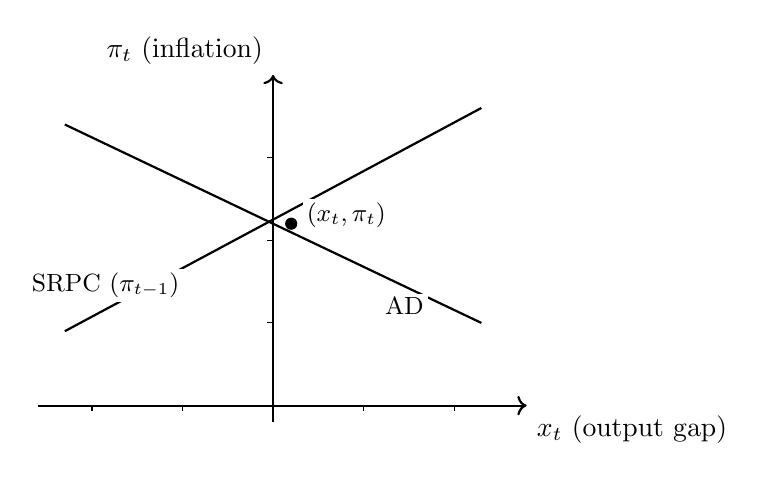
\begin{tikzpicture}[x=1.15cm,y=1.05cm]
  \xpiaxes

  % AD downward
  \draw[curve] (-2.3,3.4) -- (2.3,1.0);
  \node[lab] at (1.45,1.20) {AD};

  % SRPC upward
  \draw[curve] (-2.3,0.9) -- (2.3,3.6);
  \node[lab] at (-1.85,1.45) {SRPC ($\pi_{t-1}$)};

  % Intersection
  \coordinate (E) at (0.20,2.20);
  \fill (E) circle (2.2pt);
  \node[lab,anchor=west] at ($(E)+(0.12,0.10)$) {$(x_t,\pi_t)$};
\end{tikzpicture}
\end{column}

\begin{column}{0.38\textwidth}
\small
\begin{itemize}
\item AD: higher $\pi$ triggers tighter policy $\Rightarrow$ lower $x$.
\item SRPC: higher $x$ raises $\pi$ relative to $\pi_{t-1}$.
\item Given $\pi_{t-1}$, intersection pins today’s $(x_t,\pi_t)$.
\end{itemize}
\end{column}
\end{columns}
\end{frame}

%------------------------------------------------
\begin{frame}{Demand shock: AD shifts}
\begin{columns}
\begin{column}{0.62\textwidth}
\centering
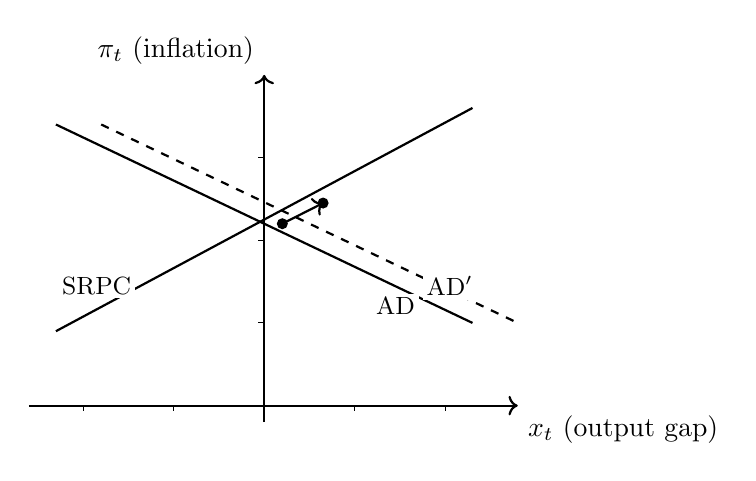
\begin{tikzpicture}[x=1.15cm,y=1.05cm]
  \xpiaxes

  % SRPC fixed
  \draw[curve] (-2.3,0.9) -- (2.3,3.6);
  \node[lab] at (-1.85,1.45) {SRPC};

  % AD baseline
  \draw[curve] (-2.3,3.4) -- (2.3,1.0);
  \node[lab] at (1.45,1.20) {AD};

  % AD' shifted right
  \draw[dashcurve] (-1.8,3.4) -- (2.8,1.0);
  \node[lab] at (2.05,1.45) {AD$'$};

  % intersections
  \coordinate (E0) at (0.20,2.20);
  \fill (E0) circle (2.0pt);
  \coordinate (E1) at (0.65,2.45);
  \fill (E1) circle (2.0pt);
  \draw[->,thick] (E0) -- (E1);
\end{tikzpicture}
\end{column}

\begin{column}{0.38\textwidth}
\small
\begin{itemize}
\item $\bar x_t\uparrow$ shifts AD right.
\item Equilibrium: $x_t\uparrow$ and $\pi_t\uparrow$.
\end{itemize}
\end{column}
\end{columns}
\end{frame}

%------------------------------------------------
\begin{frame}{Supply shock: SRPC shifts}
\begin{columns}
\begin{column}{0.62\textwidth}
\centering
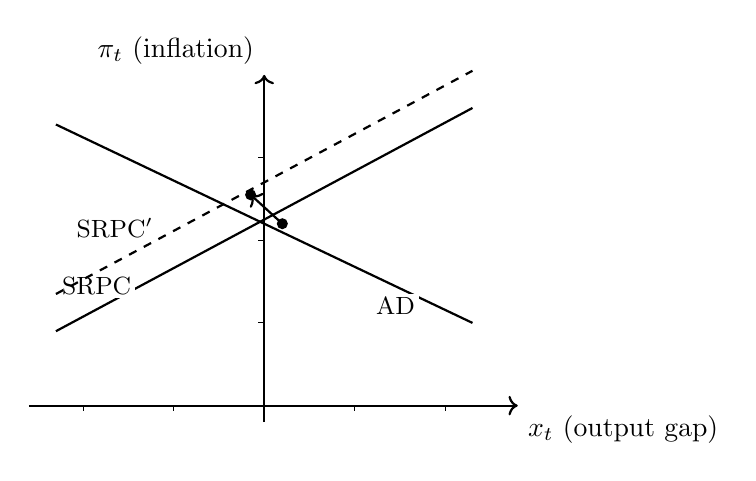
\begin{tikzpicture}[x=1.15cm,y=1.05cm]
  \xpiaxes

  % AD fixed
  \draw[curve] (-2.3,3.4) -- (2.3,1.0);
  \node[lab] at (1.45,1.20) {AD};

  % SRPC baseline
  \draw[curve] (-2.3,0.9) -- (2.3,3.6);
  \node[lab] at (-1.85,1.45) {SRPC};

  % SRPC' shift up
  \draw[dashcurve] (-2.3,1.35) -- (2.3,4.05);
  \node[lab] at (-1.65,2.15) {SRPC$'$};

  % intersections
  \coordinate (E0) at (0.20,2.20);
  \fill (E0) circle (2.0pt);
  \coordinate (E1) at (-0.15,2.55);
  \fill (E1) circle (2.0pt);
  \draw[->,thick] (E0) -- (E1);
\end{tikzpicture}
\end{column}

\begin{column}{0.38\textwidth}
\small
\begin{itemize}
\item $u_t>0$ shifts SRPC up.
\item Equilibrium: $\pi_t\uparrow$ and $x_t\downarrow$ (stagflation).
\end{itemize}
\end{column}
\end{columns}
\end{frame}

%------------------------------------------------
\section{Dynamics}

%------------------------------------------------
\begin{frame}{What carries over to the next period?}
\begin{itemize}
\item In the Phillips curve, the intercept is $\pi_{t-1}$.
\item After we determine $\pi_t$, that becomes the new intercept next period.
\item So inflation today affects inflation tomorrow even if shocks disappear.
\end{itemize}
\end{frame}

%------------------------------------------------
\begin{frame}{A consistent ``next period'' picture}
\begin{columns}
\begin{column}{0.62\textwidth}
\centering
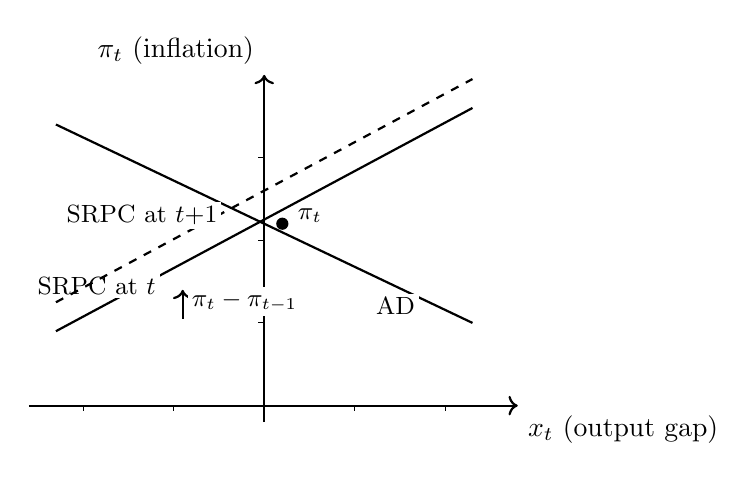
\begin{tikzpicture}[x=1.15cm,y=1.05cm]
  \xpiaxes

  % AD fixed
  \draw[curve] (-2.3,3.4) -- (2.3,1.0);
  \node[lab] at (1.45,1.20) {AD};

  % SRPC t
  \draw[curve] (-2.3,0.9) -- (2.3,3.6);
  \node[lab] at (-1.85,1.45) {SRPC at $t$};

  % equilibrium
  \coordinate (Et) at (0.20,2.20);
  \fill (Et) circle (2.2pt);
  \node[lab,anchor=west] at ($(Et)+(0.12,0.10)$) {$\pi_t$};

  % SRPC t+1 shifted up if pi_t>pi_{t-1}
  \draw[dashcurve] (-2.3,1.25) -- (2.3,3.95);
  \node[lab] at (-1.35,2.30) {SRPC at $t{+}1$};

  \draw[->,thick] (-0.9,1.05) -- (-0.9,1.40);
  \node[lab,anchor=west] at (-0.85,1.26) {$\pi_t-\pi_{t-1}$};
\end{tikzpicture}
\end{column}

\begin{column}{0.38\textwidth}
\small
\begin{itemize}
\item If $x_t>0$, the Phillips curve implies $\pi_t>\pi_{t-1}$.
\item Then next period starts from a higher intercept.
\item This is the model’s basic persistence mechanism.
\end{itemize}
\end{column}
\end{columns}
\end{frame}

%------------------------------------------------
\begin{frame}{Eliminate $x_t$: inflation follows an AR(1)}
\small
\[
x_t = \bar x_t - \eta(\pi_t-\pi^\ast),\qquad
\pi_t = \pi_{t-1} + \kappa x_t + u_t.
\]
Plug in:
\[
(1+\kappa\eta)\pi_t = \pi_{t-1} + \kappa\eta\pi^\ast + \kappa\bar x_t + u_t,
\]
\[
\Rightarrow\quad
\pi_t = \underbrace{\frac{1}{1+\kappa\eta}}_{a<1}\pi_{t-1} + (1-a)\pi^\ast
      + \frac{\kappa}{1+\kappa\eta}\bar x_t + \frac{1}{1+\kappa\eta}u_t.
\]
\end{frame}

%------------------------------------------------
\begin{frame}{Policy aggressiveness and persistence}
\small
\[
a=\frac{1}{1+\kappa\eta},\qquad
\eta=\frac{\sigma\phi_\pi}{1+\sigma\phi_x}.
\]
\begin{itemize}
\item Larger $\phi_\pi$ $\Rightarrow$ larger $\eta$ $\Rightarrow$ smaller $a$.
\item Translation: stronger inflation targeting makes inflation return faster toward target.
\item Cost-push shocks $u_t$ raise inflation on impact even if demand is weak.
\end{itemize}
\end{frame}

%------------------------------------------------
\section{Wrap-up}

%------------------------------------------------
\begin{frame}{Checklist for reading a shock episode with this model}
\begin{enumerate}
\item Identify which curve moved: AD ($\bar x_t$) or SRPC ($u_t$).
\item Use the intersection picture to infer $(x_t,\pi_t)$.
\item Use the AR(1) to discuss persistence (role of $a$).
\item Connect policy talk to parameters ($\phi_\pi,\phi_x$).
\end{enumerate}
\end{frame}

%------------------------------------------------
\begin{frame}{Preview of the next step}
\begin{itemize}
\item Replace backward-looking inflation with forward-looking pricing (New Keynesian).
\item Revisit what ``policy stabilizes inflation'' means when expectations are forward-looking.
\end{itemize}
\end{frame}

\end{document}
